\documentclass[11pt]{article}

\usepackage[utf8]{inputenc}
\DeclareUnicodeCharacter{2212}{\ensuremath{-}}
\usepackage[margin=1in]{geometry}
\usepackage{booktabs}
\usepackage{float}
\usepackage{microtype}
\usepackage{parskip}
\usepackage{graphicx}
\usepackage{enumitem}
\usepackage[font=small,labelfont=bf,margin=0.5em]{caption}
\usepackage[numbers,sort&compress]{natbib}
\setcitestyle{super,open={[},close={]}}
\usepackage{placeins}
\usepackage{xcolor}
\usepackage[hidelinks]{hyperref}
\usepackage{xurl}

\title{\vspace{-1.5em}Crowdsourced Mosquito Sightings as an Early Signal of West Nile Virus}
\author{Alexander Pirouznia \\ \small arp286 \and Pratheet Joshi \\ \small paj54 \and Sriram Sundararajan \\ \small ss4598}
\date{CS/INFO 5306 \\ 11/09/2026}

\begin{document}
\maketitle

\section{Introduction}
West Nile virus (WNV) was found in the United States for the first time in 1999. The first year, CDC records show 62 human cases, and within four years the virus had spread across the country. In 2003 alone the CDC recorded 9,862 cases,\cite{cdc_historic} and it has stayed ever since. Between 2016 and 2025, ArboNET, the national arboviral surveillance system run by the CDC and state health departments, recorded 19,232 human cases, 13,063 of which were neuroinvasive.\cite{cdc_historic}

Around a decade later, a group of graduate students at UC Berkeley launched a master's final project called iNaturalist,\cite{inat_about} where anyone could photograph a plant or animal, upload it with a time and a place, and let a community of naturalists help identify it. The project has since grown into one of the world's largest biodiversity platforms, and its users now photograph mosquitoes along with everything else. None of these users are trying to do disease surveillance.

This brings us to our core research question: can the mosquito sightings that iNaturalist users post for biodiversity reasons act as an early signal of West Nile virus activity? More specifically, does an unusually mosquito-heavy spring on iNaturalist precede a worse WNV season in the same place? The hypothesis that we had and intended to test was that it would, and that the signal would be strongest for mosquitoes of the genus \textit{Culex}, which are the main carriers of the virus.

In doing so, we find that the answer is mostly no. Mosquito-heavy seasons on iNaturalist tend to be worse WNV seasons nationally, but the crowd signal does not tell you which states or counties are in for a bad year and it adds no forecasting skill beyond a state's own history. We then repeated the test at a finer scale using weekly county data from California and Texas. California gave the same answer, while Texas showed a small association between sightings and later WNV-positive mosquito pools, but one that was too flat and too weak where it mattered to work as a warning.

\section{Background}
West Nile virus cycles between birds and mosquitoes and especially \textit{Culex} species. Some infected birds develop high levels of virus in their blood, mosquitoes that bite them become infected, and those mosquitoes can then pass the virus on to more birds and eventually to people.\cite{cdc_causes} This is what made the idea plausible to us in the first place: if more mosquitoes are around and noticeable, more people might photograph them, and more transmission might follow.

The idea of finding a disease signal in online behavior is not new, and Ginsberg et al.\ showed that Google search queries could track influenza-like illness one to two weeks ahead of CDC reports.\cite{ginsberg2009} Goel et al.\ later argued that a signal like this is only useful if it beats a simple baseline and found that a plain model did almost as well as search data for flu.\cite{goel2010} Our crowd signal comes from a source that was never meant for epidemiology and we judged it against the simplest baseline we could think of, which is what each state's WNV level usually is.

\section{Online Data and Resources}
In order to begin collection of our data, we used the iNaturalist API\cite{inat_api} through a series of Python scripts. We pulled every verifiable US observation of the mosquito family (Culicidae) from 2015 through 2025, which came out to 76,129 observations posted by 23,144 different people. For each observation we kept the date, an anonymous observer ID, the taxon it was identified as, its quality grade, and its coordinates.

A count of mosquito photos on its own does not mean much without knowing how many people were out photographing insects in general, so we also pulled denominators from the API's histogram endpoint. These were monthly counts per state of all insect observations (about 30 million in total), of crane-fly observations, and of all observations, as well as yearly insect counts for each of the 2,357 counties where at least one mosquito had been recorded.

For West Nile virus, we used the CDC's ArboNET historic data.\cite{cdc_historic} The dashboard on that page is built on downloadable files that give human cases, neuroinvasive cases and non-human activity for every county and year from 1999 to 2025, and national case counts by month of illness onset. We chose neuroinvasive cases as our outcome because the CDC itself notes that milder cases are under-reported unevenly and should not be compared across places or over time.\cite{cdc_historic} Finally, we used 2016 Census county population estimates\cite{plotly_county} to turn county case counts into incidence rates.

To link the two sources, we placed each mosquito observation in a county by matching its coordinates against Census county boundaries. For the observations whose exact location iNaturalist hides for privacy, we used iNaturalist's own county assignment instead. As a validation step, our state totals came within 0.3\% of iNaturalist's own counts and our county case totals added up exactly to the national totals the CDC publishes (for example, 2,167 cases and 1,517 neuroinvasive cases in 2025).

The national data cannot say when in a season cases begin, so we added two sources that report weekly by county. For California, we used the California Department of Public Health's human case file, keeping 2019 through 2025.\cite{cdph_wnv} For Texas, we used weekly reports that the Texas Department of State Health Services publishes as PDFs, reading the county table out of all 585 of them and subtracting consecutive weeks to get new counts.\cite{dshs_weekly} Because Texas hides counties with fewer than 5 human cases in a year, we used WNV-positive mosquito pools as its outcome, which are far more numerous than human cases and turn positive before people get sick. We checked our totals against each report's own summary table, and they matched in all but one week. For both states we pulled mosquito and total observations for every county and week from the same API.\cite{inat_api}

\section{Our Original Question and How It Changed}
Our proposal asked whether spatiotemporal sightings of \textit{Culex} mosquitoes could predict WNV cases at the level of a county-week. We planned to compare several crowd measures, namely raw observation counts, the number of unique observers, changes from a location's normal level, and mosquito observations as a share of local iNaturalist activity. Once we actually had the data, three problems forced us to change the question.

\begin{enumerate}[leftmargin=*]
\item \textbf{\textit{Culex} is too rare a label.} Only 10.0\% of mosquito observations were identified as \textit{Culex} (7,585 over ten years). Most of what people photograph is \textit{Aedes} (39.6\%) or \textit{Psorophora} (11.9\%), and another 11.7\% are never identified past the family level. We therefore made all mosquitoes our main signal and kept \textit{Culex} as a sub-signal.
\item \textbf{County-weeks are almost always empty.} The median county has only 6 mosquito observations in ten years, and only 2.6\% of county-weeks have any at all. Even Cook County, Illinois, home to Chicago, has 479. On top of this, the CDC's public data only goes down to county-year, and the timing of illness onset is only published nationally by month. We moved to state-years (50 states and DC over ten years), national months, and a pooled comparison across counties.
\item \textbf{Raw counts measure the app, not the mosquitoes.} Mosquito observations grew from 1,156 in 2016 to 16,770 in 2025, roughly fourteen-fold, while WNV cases showed no trend at all (Figure~\ref{fig:growth}). To deal with this, we divided each mosquito count by the number of insect observations from the same place and months, which we call the mosquito share, and we compared every state against its own normal level and against the national year.
\end{enumerate}

\begin{figure}[htbp]
\centering
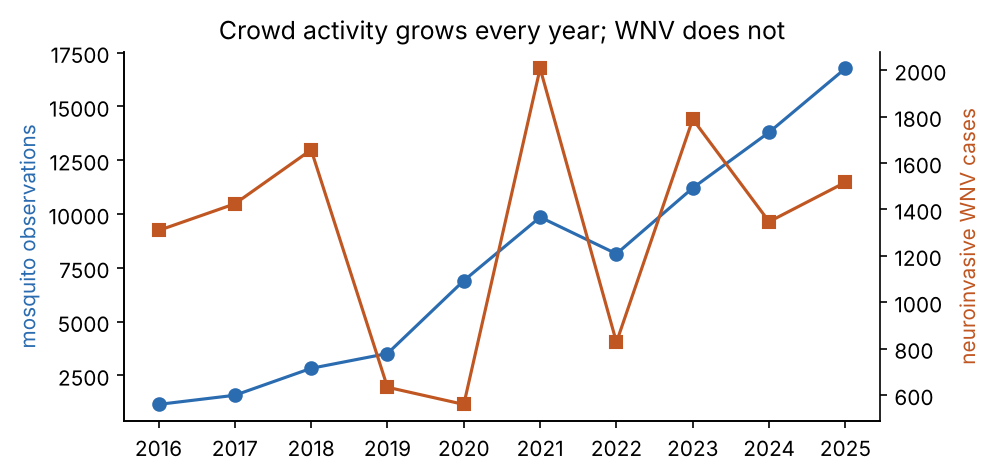
\includegraphics[width=0.78\textwidth]{figures/fig1_growth}
\caption{Mosquito observations on iNaturalist per year (blue) against neuroinvasive WNV cases reported to the CDC (orange), 2016--2025. Crowd activity grows every year while WNV moves up and down.}
\label{fig:growth}
\end{figure}

The question we ended up asking was this: within a state, does an April--July mosquito share that is higher than usual, in a year that is not unusual nationally, go along with more neuroinvasive WNV cases that year? We picked April through July because human cases peak in August and September, so a signal from those months would have to come first. Alongside this main test, we also asked whether mosquito sightings lead cases over the course of a season, whether mosquito-heavy years are worse WNV years nationally, and whether counties with a higher mosquito share see more WNV. We kept the proposal's other crowd measures as alternatives, and we added crane flies, a common mosquito look-alike that carries no disease, as a placebo. After finishing this national analysis, we went back to the proposal's county-week design in the two states whose health departments publish weekly data, which is described below.

\section{Methods}
Our mosquito share was computed as (mosquito observations + 0.5) divided by (insect observations + 1), so that a state with no mosquito photos in a given window would not produce a zero, and we analyzed it on a logarithmic scale. The outcome was log(1 + neuroinvasive cases). For the main test, we fit a regression of the outcome on each April--July crowd signal with fixed effects for each state and each year, and clustered the standard errors by state. Importantly, the state effects absorb how WNV-prone a state normally is and how popular iNaturalist is there, while the year effects absorb nationally good and bad seasons. We only kept state-years with at least 200 insect observations in April--July, which removed 2 of the 510.

We also ran a number of robustness checks. These included restricting to 2020--2025 when iNaturalist volume was large, a negative binomial model on the raw case counts, a version without year effects, and within-state rank correlations for each state. Following the lesson from Goel et al., we ran a leave-one-year-out forecast in which each state's season was predicted either from that state's average in the other years alone, or from that average plus the mosquito anomaly, and compared the errors.

At the national level, we built monthly anomalies for May through October by subtracting each calendar month's ten-year average from both the mosquito share and the case counts. Since ten seasons is not a lot of data, we tested these correlations with a permutation test that shuffles which year's mosquito series is paired with which year's cases. For counties, we pooled 2016--2025 and compared the mosquito share with average annual incidence across 2,160 counties that had at least 300 insect observations, controlling for population, overall insect activity and state. We left out Connecticut because its county codes changed in 2022.

For the weekly data we followed the proposal more closely and worked at the level of the county-week. In California, we compared each county's weekly mosquito share with its usual level for that week and checked whether it lined up with cases zero to eight weeks later, using the same year-shuffling test as at the national level to judge chance. In Texas, county-weeks were so sparse that we pooled each signal over four weeks, and we kept the 35 counties with at least one positive pool and enough iNaturalist activity, which hold 99\% of all positive pools. We then compared new positive pools with the mosquito share from zero to ten weeks earlier, with effects for each county's usual season and for each week of each year, so that only a county's departure from its own normal counts. We checked this against a placebo that pairs each county with a different year's pools, controlled for the county's own pool history, and ran the same leave-one-year-out forecast as before. Texas has no insect count, so its share is out of all observations.

\section{Results}
The results we found mostly did not support our hypothesis. Every mosquito signal pointed in the direction we expected, but in the national data none of them held up once we accounted for what a state's WNV level usually is, and the weekly California data did not do better. Texas was the one partial exception.

\subsection{Seasonal timing}
Mosquito observations center on mid-July, about 1.1 months before the center of neuroinvasive onsets in mid-August (Figure~\ref{fig:national}a). At first glance this looks like a lead, but insect observations in general center on early July, so most of this lead is simply when people are outside taking pictures of bugs. Mosquito observations also stay roughly flat from June through September rather than climbing toward the WNV peak. Surprisingly, \textit{Culex} observations peak in October, when 16.5\% of them were posted, which is after the August peak that holds 38.9\% of onsets. One possible explanation is that \textit{Culex} females come indoors in the fall to wait out the winter, where people are more likely to notice them.

\begin{figure}[htbp]
\centering
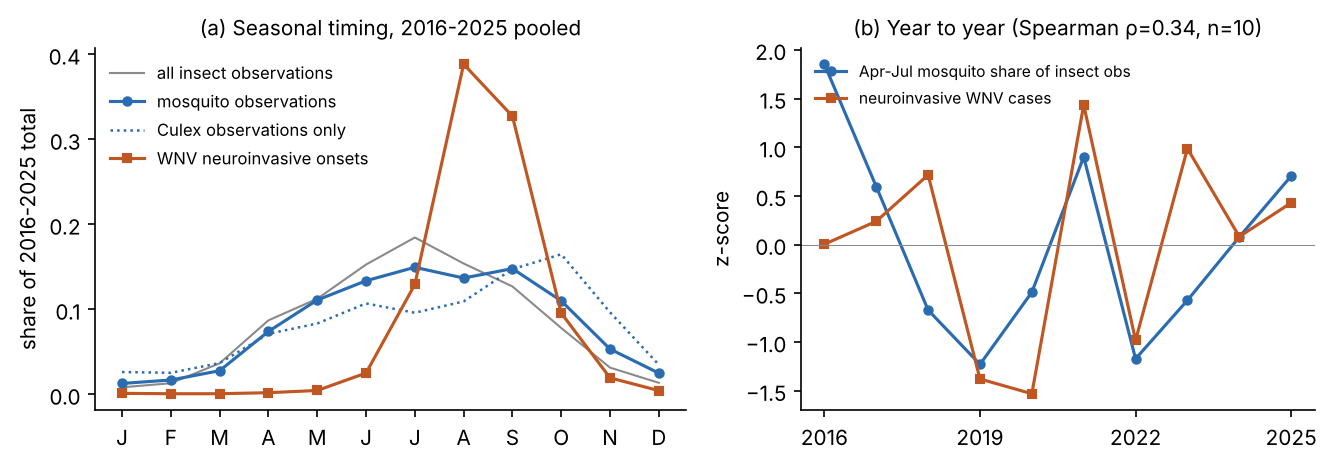
\includegraphics[width=\textwidth]{figures/fig2_national}
\caption{(a) Share of all 2016--2025 records falling in each calendar month for insects, mosquitoes, \textit{Culex} and neuroinvasive WNV onsets. (b) Year-to-year z-scores of the national April--July mosquito share and neuroinvasive cases.}
\label{fig:national}
\end{figure}

\subsection{Year to year nationally}
At the national level, there is a real but loose link. The April--July mosquito share and that year's neuroinvasive cases had a rank correlation of 0.35 (p = 0.33, n = 10), and the July--September share did better at 0.58 (p = 0.08) (Figure~\ref{fig:national}b). With the monthly anomalies, a mosquito share above its usual level was followed by more cases one and two months later (r = 0.39 and 0.44), and this survived the permutation test (p = 0.02 for both). However, when we also removed each year's average, the correlation dropped to between 0.05 and 0.15 and was no longer significant. This told us that the link is about whole seasons being mosquito-heavy, and not about month-to-month timing within a season.

\subsection{State-year panel}
Table~\ref{tab:panel} shows the main test. Every mosquito signal has a positive coefficient and the crane-fly placebo has a negative one, but none of them are significant, and none explain even 1\% of the variation that is left after state and year effects. Counting unique observers instead of observations did not help, and neither did narrowing down to \textit{Culex}. Figure~\ref{fig:panel} shows how little the mosquito signal stands out from the placebo.

\begin{table}[htbp]
\centering
\small
\begin{tabular}{lcccc}
\toprule
April--July signal & Coefficient & SE & p & Within-$R^2$ \\
\midrule
Mosquito share of insect observations & 0.072 & 0.063 & 0.25 & 0.003 \\
Mosquito observers per insect observation & 0.058 & 0.089 & 0.51 & 0.001 \\
\textit{Culex} share of insect observations & 0.050 & 0.038 & 0.19 & 0.003 \\
Raw mosquito observations (log) & 0.090 & 0.073 & 0.22 & 0.005 \\
Unique mosquito observers (log) & 0.098 & 0.106 & 0.35 & 0.003 \\
Placebo: crane-fly share & $-$0.058 & 0.086 & 0.50 & 0.001 \\
Mosquito share, full year (concurrent) & $-$0.005 & 0.065 & 0.93 & 0.000 \\
\bottomrule
\end{tabular}
\caption{Regressions of log(1 + neuroinvasive cases) on each crowd signal with state and year fixed effects, 508 state-years, standard errors clustered by state. Within-$R^2$ is the share of variation explained beyond the state and year effects.}
\label{tab:panel}
\end{table}

\begin{figure}[htbp]
\centering
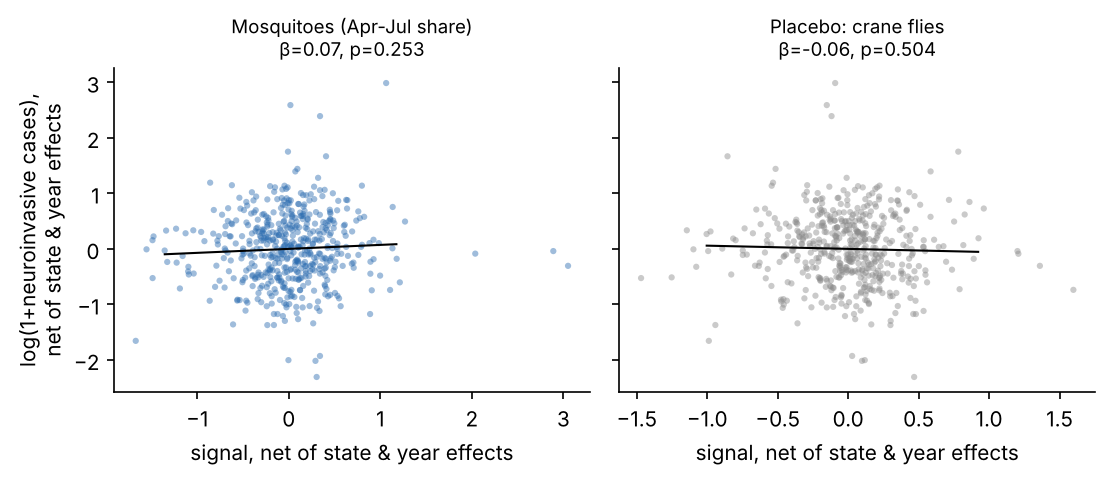
\includegraphics[width=0.9\textwidth]{figures/fig3_panel}
\caption{April--July signal against neuroinvasive cases, both net of state and year effects, for mosquitoes (left) and the crane-fly placebo (right). Each point is one state-year.}
\label{fig:panel}
\end{figure}

The robustness checks told the same story. Restricting to 2020--2025, when iNaturalist had enough users for state shares to be stable, gave the strongest result at 0.25, but it still was not significant (p = 0.08, 306 state-years). The negative binomial model gave a coefficient of 0.20, which looks significant with the model's own standard errors (p = 0.01) but not once they are clustered by state (p = 0.10). Removing the year effects made the signal significant (0.13, p = 0.03), which matches what we saw nationally: the signal appears once nationally bad years are allowed to count. State by state, 28 of 46 states had a positive within-state correlation, which is not much better than a coin flip (sign test p = 0.18). Most telling of all, adding the mosquito anomaly to a state's own average made the leave-one-year-out forecasts slightly worse rather than better, with a mean absolute error of 0.687 compared to 0.682.

We also ran into the trap that the raw counts set. Pooled across all state-years, raw mosquito counts correlate with cases at 0.23 (p $<$ 0.001), which could easily be mistaken for a finding. Once the counts are turned into a share, this drops to $-$0.04, because large states simply have more of both.

\subsection{Counties}
Counties with a higher mosquito share do have slightly higher average neuroinvasive incidence (rank correlation 0.066, p = 0.002) and more years with any WNV activity (0.075, p $<$ 0.001). However, once we compared counties only within their own state and controlled for population and insect activity, the effect vanished (coefficient 0.006, p = 0.57). The raw correlation reflects which states are prone to WNV, not anything happening locally (Figure~\ref{fig:county}).

\begin{figure}[htbp]
\centering
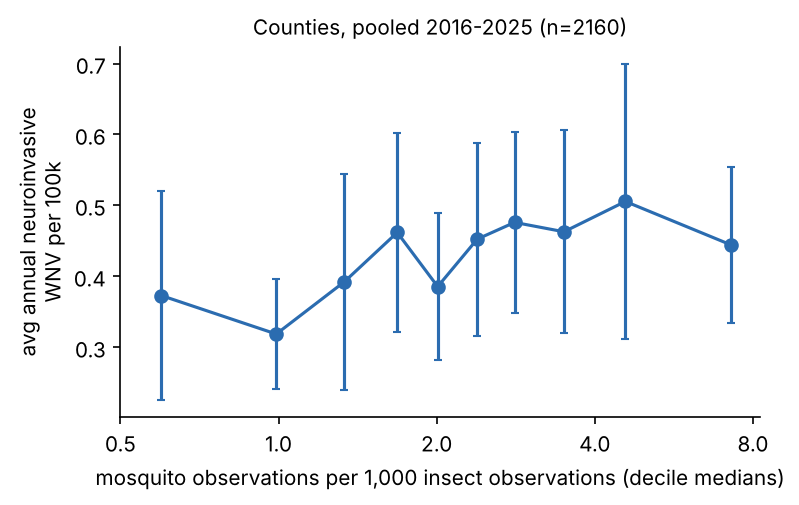
\includegraphics[width=0.7\textwidth]{figures/fig4_county}
\caption{Average annual neuroinvasive WNV incidence per 100,000 people by decile of a county's mosquito share, pooled 2016--2025, with 95\% intervals.}
\label{fig:county}
\end{figure}

\subsection{Weekly data from California and Texas}
Moving to weekly data in California did not change the answer. Only 18\% of the state's sightings are identified as \textit{Culex}, and the San Joaquin Valley counties, which are among the places with the most WNV, have sightings in only a small share of weeks. After removing seasonality, the best correlations between weekly sightings and cases up to eight weeks later were about 0.10 to 0.25, and none clearly beat chance in the year-shuffling test. Years when a county's spring sightings ran above its norm did not have more cases that fall either. Sacramento shows how easily a signal can be faked (Figure~\ref{fig:ca}). Its fall 2023 spike in sightings lined up with a spike in cases, but one user posted 348 of the 351 sightings, and the correlation of about 0.30 fell to around 0.10 once we counted unique observers.

\begin{figure}[htbp]
\centering
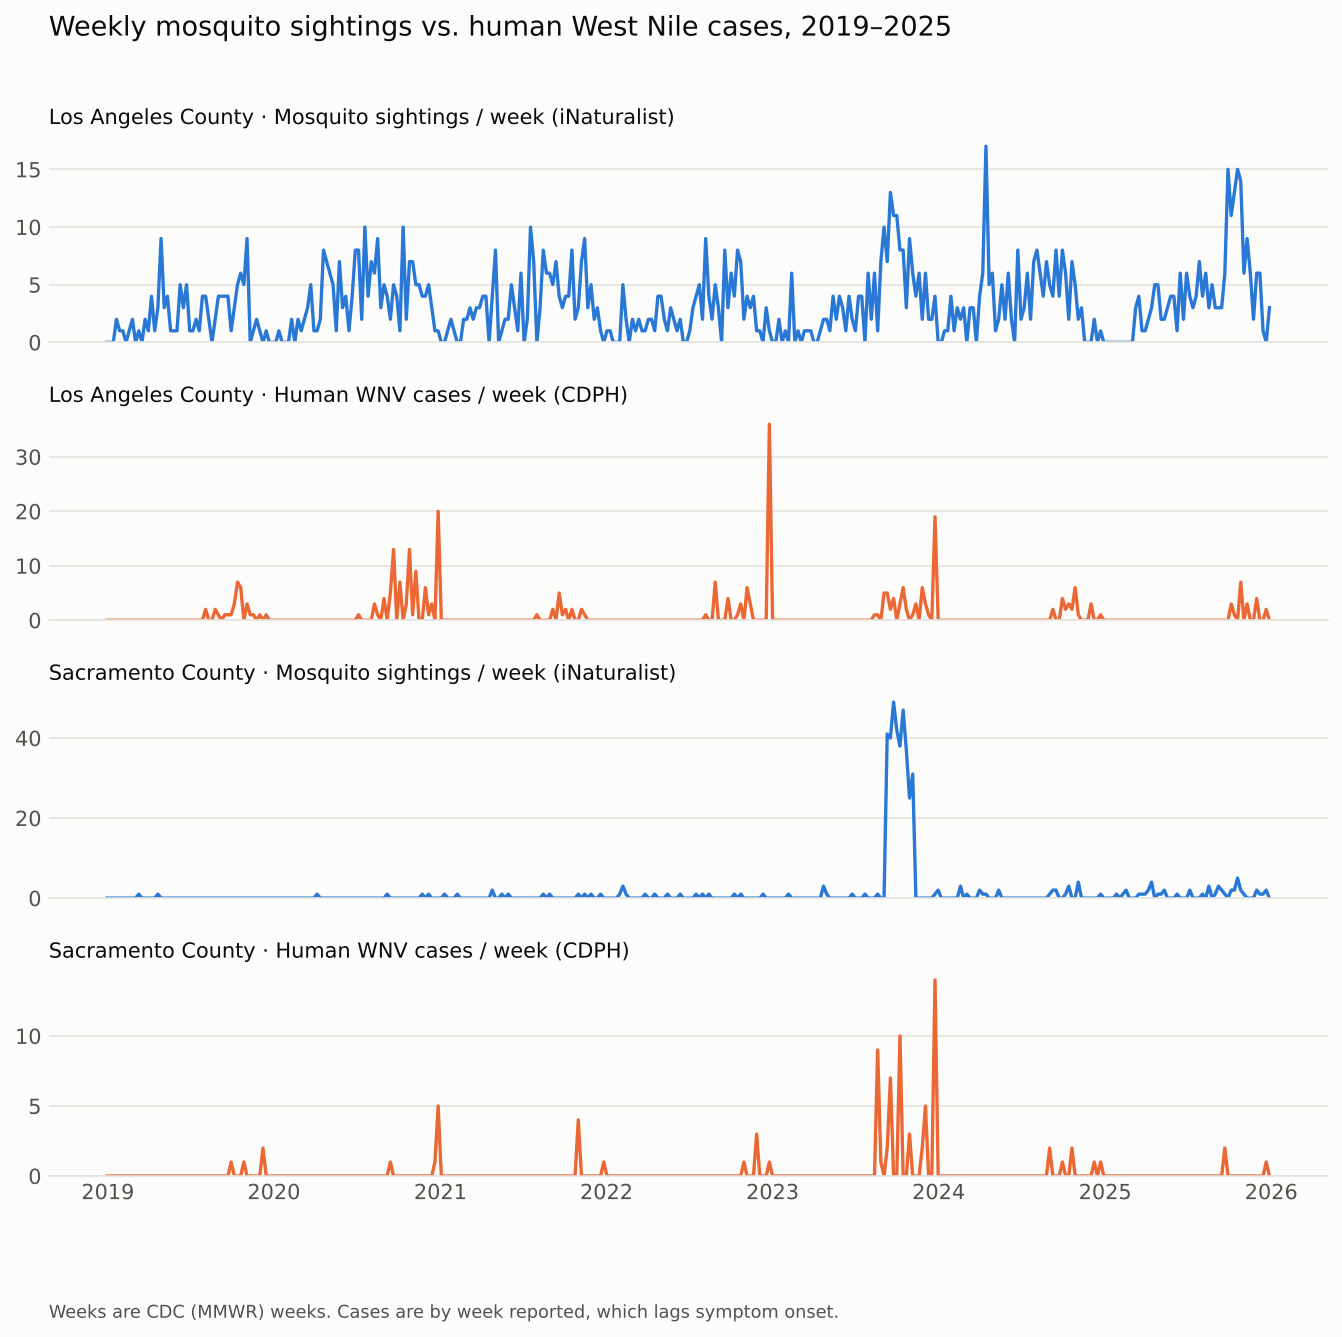
\includegraphics[width=0.85\textwidth]{figures/timing_la_sacramento}
\caption{Weekly mosquito sightings (blue) and human WNV cases by week of report (orange) for Los Angeles and Sacramento counties, 2019--2025. Sacramento's fall 2023 spike in sightings came from a single user.}
\label{fig:ca}
\end{figure}

Texas is the one place where we found something. In the 35 counties we analyzed, a county with more mosquito sightings than usual had somewhat more positive mosquito pools in the following weeks, and the link was strongest from three weeks on (Figure~\ref{fig:tx}). It remained when we paired each county with a different year's pools (p = 0.002) and when we accounted for the county's own pool history, but it did not appear for human cases at any lead. It is also small, since most county-weeks have no new positive pool at all.

\begin{figure}[htbp]
\centering
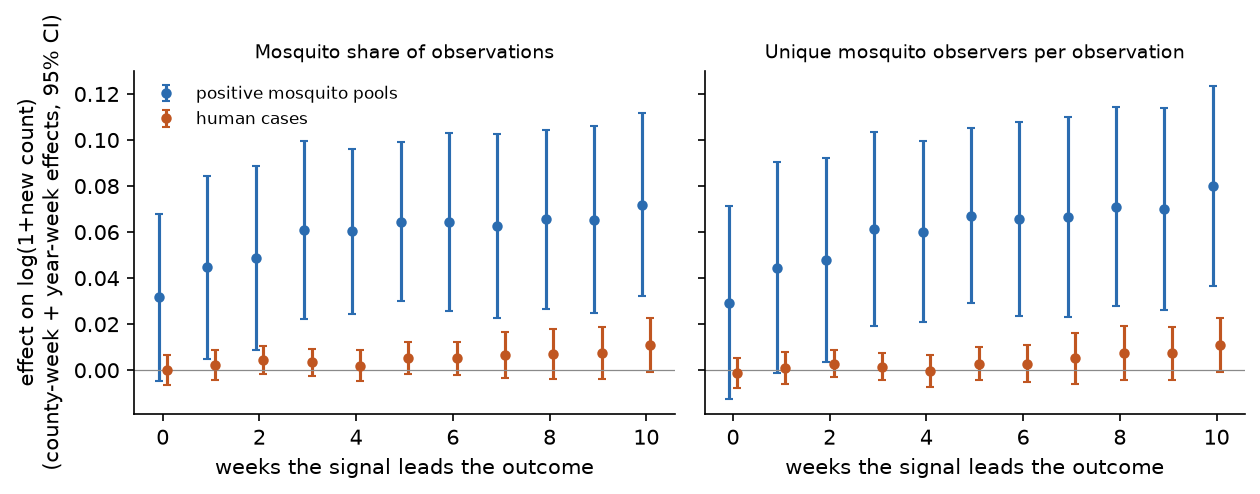
\includegraphics[width=\textwidth]{figures/tx_lags}
\caption{Effect of the Texas mosquito signal on positive pools (blue) and human cases (orange) by how many weeks the signal leads, with 95\% intervals. Left: mosquito share of observations. Right: unique mosquito observers per observation.}
\label{fig:tx}
\end{figure}

We do not read this as an early warning, for three reasons. The effect rises until about three weeks and then stays flat out to ten weeks, which looks more like counties and seasons that are busy for both than a signal that arrives first. It is also missing in the ten counties with the most pools, which are the places where a forecast would matter most, and it did not appear for \textit{Culex} alone. Finally, adding sightings to a county's own history improved its forecast by only 2.5\%.

\FloatBarrier
\section{Discussion}
As mentioned earlier in our paper, the crowd signal we found shows up across whole national seasons and, in Texas, as a small association with positive mosquito pools, but it does not tell us which places or weeks are about to get worse. One possible explanation for this is what people actually photograph, because the observations are dominated by \textit{Aedes} and \textit{Psorophora}, and the \textit{Culex} mosquitoes that carry the virus make up only a tenth of them and are posted most often in the fall, which is after the outbreak has already peaked. In other words, the crowd is documenting the mosquitoes that bother them and not the ones that are relevant for WNV.

It is also worth noting that the crowd itself was not the problem nationally. The 75,798 mosquito observations from 2016--2025 came from 23,078 people, 69.4\% of whom posted only one mosquito, and the top ten users accounted for only 5.5\% of observations.

Texas is where the hypothesis came closest to working. Positive pools are the outcome nearest to the mosquitoes themselves, so it is not surprising that a crowd report about mosquitoes lines up with them better than with human cases. One possible explanation for why this still falls short of a warning is that both pools and sightings depend on how many people are paying attention, since traps have to be set and tested just as photos have to be taken. In other words, the crowd may be partly measuring attention instead of mosquitoes.

These findings may have broader implications for using citizen science as a public health signal. A platform like iNaturalist can tell us when and roughly where people are noticing mosquitoes, so in a sense that does line up with bad WNV years. However, the step from ``people noticed more mosquitoes'' to ``more people got sick here'' requires the right species, at the right time, in the right place, and our data was thin on all three. Like Goel et al.\ found with search data, the signal only looks impressive until it is compared to a simple baseline.\cite{goel2010}

That said, something of note that can be expanded on with further analysis is the national pattern. A hot summer could possibly produce both more noticeable mosquitoes and more WNV transmission at once, which may explain why the link shows up across whole seasons but not within states. Testing this would require weather data, which was outside the scope of this project. A more targeted design, such as focusing only on research-grade \textit{Culex} observations or adding the number of mosquito traps set each week in Texas, might also show a sharper signal.

\section{Limitations and Conclusion}

\subsection{Limitations}
The biggest limitation of our study is power, since ten years means only ten national seasons. In 2016 the entire country logged 535 mosquito observations between April and July, so state shares before about 2019 are mostly noise. The CDC only publishes onset timing nationally and only yearly totals by state and county, so the national analysis could not test a lead at the state-week level. The weekly data from California and Texas let us do so, but their dates are when a case or pool was reported rather than when it began, which blurs any lead. Seven seasons is also a short record, and since we tried many leads, the Texas p-values are optimistic. Cases are also counted by county of residence rather than where the person was bitten, which blurs the county comparison. On the iNaturalist side, 60\% of the observations have not reached research grade, which means that the community has not yet agreed on their identification. Finally, our county boundaries were generalized, which may misplace a small number of observations near county lines, and our county populations are from a single year.

\subsection{Conclusion}
iNaturalist users posted over 76,000 mosquito observations in the US without ever trying to track a disease, and in a broad sense their activity does line up with West Nile virus: mosquito-heavy seasons nationally tend to be worse WNV seasons. Within a state, an unusually mosquito-heavy spring did not predict a worse season, \textit{Culex} sightings were too rare and came too late, and adding the crowd signal made forecasts slightly worse than simply using a state's history. Weekly county data did not support the idea either. In California, sightings did not clearly come before cases, and in Texas they were followed by somewhat more positive mosquito pools, but only weakly, not in the counties with the most pools, and not for human cases. That suggests to us that the deciding factor is less the size of the crowd and more whether the crowd is looking at the right thing.

\bibliographystyle{unsrtnat}
\bibliography{references}

\appendix
\clearpage
\renewcommand{\thesection}{\Alph{section}}
\section{Effort}
Most of our time went into getting the data and making sure the data sources lined up. The iNaturalist API limits the rate of requests, so pulling many observations, monthly histograms for every state, and yearly insect counts for counties took a good amount of time. Additionally, most of the CDC's county data lives inside an interactive dashboard, so we had to find the data files that sit behind it. We then validated both sources against their published totals.

\section{Use of AI and Other Online Resources}
We used Claude\cite{claude} to help write the data collection and analysis scripts, run the statistical analysis, and draft this report and our summary slide from our proposal and results.

Other resources: the \href{https://api.inaturalist.org/v1/docs/}{iNaturalist API}\cite{inat_api}, the \href{https://www.cdc.gov/west-nile-virus/data-maps/historic-data.html}{CDC West Nile virus historic data}\cite{cdc_historic}, documentation for \href{https://pandas.pydata.org/docs/}{pandas}\cite{pandas}, \href{https://www.statsmodels.org/stable/}{statsmodels}\cite{statsmodels}, \href{https://shapely.readthedocs.io/}{shapely}\cite{shapely} and \href{https://matplotlib.org/stable/}{matplotlib}\cite{matplotlib}, and the papers we read in class, especially \href{https://doi.org/10.1038/nature07634}{Ginsberg et al. (2009)}\cite{ginsberg2009} and \href{https://doi.org/10.1073/pnas.1005962107}{Goel et al. (2010)}\cite{goel2010}.

\end{document}
